%distanza indotta dalla metrica

\begin{figure}[h]
	\centering
	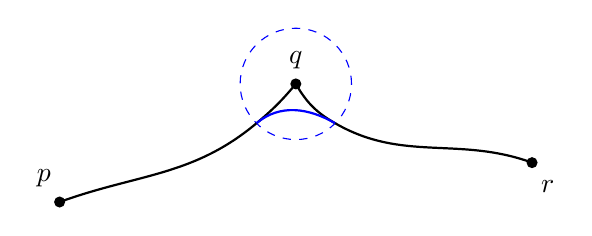
\begin{tikzpicture}
		%\draw [help lines] (-4,-2) grid (4,2);
		\fill (-3,-1)circle (2pt);
		\node at (-3.2,-0.7){\(p\)};
		\fill (0,.5) circle (2pt);
		\node at (0,0.8){\(q\)};
		\fill (3,-0.5) circle (2pt);
		\node at (3.2,-0.8){\(r\)};
		\draw[blue, dashed] (0,.5) circle (0.7071);
		\draw[thick] (-3,-1) to[out=20,in=220](-.5,0) to[out=40, in =230](0,.5) to[out=300, in=150] (.5,0) to[out=330, in=160] (3,-0.5);
		\draw[thick, blue] (-.5,0) to[out=40, in=150] (.5,0);

		
	\end{tikzpicture}
	
	\caption{Costruzione per dimostrare la disuguaglianza triangolare}
	
	\label{fig: metrica}
	
\end{figure}